\chapter{Function Algebras and Hierarchies}

\begin{quotation}

\footnotesize\sffamily\itshape

\begin{flushright}

In principle, we should be able to start with functions [...] that are so
simple that they will be unequivocally considered computable [...], and combine
them slowly and patiently through combinators that are also very elementary and
obviously computable [...] and finally get a class of functions [...] that are
quite general and nontrivial.

\smallbreak

\upshape

--- Lewis \& Papadimitriou, \emph{Elements of the Theory of Computation} (1998)

\end{flushright}

\end{quotation}

It is perhaps of interest to mathematicians et al. to categorise functions into
classes and hierarchies.

\begin{definition} A \textbf{function class}, $\mathcal{C}$, is a set of
functions. \index{function!class} \end{definition}

\begin{definition} A \textbf{function hierarchy}, $\mathcal{H}$, is a finite
sequence of $n$ classes $\mathcal{C}_1, \ldots, \mathcal{C}_n$, such that
$\mathcal{C}_1 \subseteq \cdots \subseteq \mathcal{C}_n$.
\index{function!hierarchy}\end{definition}

A class of functions can be defined \emph{extrinsically}, e.g.  the functions
computable by means of a Turing machine, or \emph{intrinsically}, e.g. the
functions contained in a function algebra.

\begin{definition} A \textbf{function algebra}, $\mathcal{F}$, is a smallest
superset of a chosen set of \textbf{initial functions} $\mathcal{F}_I$, closed
under a chosen set of operations, $\mathcal{F}_O$. An \textbf{operation} is a
(non-initial) function, which takes functions as input, and yields a function
as output. A class $\mathcal{F}$ is \textbf{closed under} an operation, if the
operation takes functions in $\mathcal{F}$ as input, and yields a function in
$\mathcal{F}$ as output. \index{function!algebra}\end{definition}

\begin{remark} That which is here called a ``function algebra'' is often simply
called a ``function class''. This is usually in the absence of an intended
distinction between an intrinsic and extrinsic definition of a function class,
which is prevalent here. For our intents and purposes, every function algebra
$\mathcal{F}$ defines a function class $\mathcal{C}$, but not every function
class is given by a function algebra.  \end{remark} 

\section{A ``simple'' function algebra}

The following simple function algebra forms the basis of many function classes
and hierarchies going forth. It boasts two ``simple'' initial functions:

\begin{definition} \label{def:zero-function} Let $z : S \rightarrow \mathbb{N}$
be a (constant) \textbf{zero function}, for any given set $S$, given by $z\p{x}
= 0$, for all $x \in S$.  \index{function!zero} \end{definition}

\begin{definition} \label{def:successor-function} Let $s : \mathbb{N}
\rightarrow \mathbb{N}$ be a \textbf{successor function}, given by $s\p{n} = n
+ 1$, for all $n \in \mathbb{N}$. \index{function!successor} \end{definition}

Furthermore, it is closed under the following ``simple''\footnote{What is meant
by``simple'' is clarified at the end of this section.} operation:

\begin{definition} \label{def:composition-operation} Let\begin{align*}
%
\circ^n_m : \p{T_1 \times \cdots \times T_m \rightarrow U} \rightarrow \p{S
\rightarrow T_1} \times \cdots \times \p{S \rightarrow T_m} \rightarrow \p{S
\rightarrow U}
%
\end{align*}be a \textbf{composition} (also called substitution)
\textbf{operation}, which takes as input a \textbf{composition operator} $g :
T_1 \times \cdots \times T_m \rightarrow U$ and $m$ \textbf{composition
operands} $h_1 : S \rightarrow T_1$, \ldots, $h_m : S \rightarrow T_m$, and
yields as output the \textbf{composite function} $f : S \rightarrow U$,
satisfying the equation\begin{align*}
%
f\p{x_1,\ldots,x_n} = g\p{h_1\p{x_1,\ldots,x_n}, \ldots, h_m\p{x_1,
\ldots,x_n}}
%
\end{align*} The composition $\circ^n_m\p{g,h_1, \ldots, h_m}$ is also written
as $g \circ \seq{h_1, \ldots, h_m}$; in the special case that $m=1$, it is also
written as $g \circ h$.\end{definition}

To better guide the intuition about composition, it is worth noting the
following properties of any composite function $f = g \circ \seq{h_1, \ldots,
h_m}$:

\begin{enumerate}

\item $cod\p{f} = cod\p{g}$;

\item $dom\p{f} = dom\p{h_1} = \cdots = dom\p{h_m}$; and

\item $dom\p{g} = cod\p{h_1} \times \cdots \times cod\p{h_m}$.

\end{enumerate}

\begin{definition} \label{def:function-algebra-p} Let $\mathcal{PD}$ be a
\textbf{simple Peano-Dedekind function algebra}, having the zero and successor
initial functions, and closed under the composition operation.\end{definition}

For instance, $z$, $s$, $\p{s \circ z}$, $\p{s \circ \p{s \circ z}}$, as well
as, the slightly more extravagant, $\p{z \circ z}$, $\p{s \circ s}$ and $\p{z
\circ \seq{z, s, z}}$, are all functions in $\mathcal{PD}$. (The latter
examples are further illuminated below.)

More generally, a function $f \in \mathcal{F}$ is either an initial function $i
\in \mathcal{F}_I$, or the application of an operation $op \in \mathcal{F}_O$
to an adequate sequence of functions $g_1, \ldots, g_n \in \mathcal{F}$.  As
such, every function $f$, in a function algebra $\mathcal{F}$, admits an
interpretation as a construction tree $\mathcal{T}_\mathcal{F}\p{f}$:

\begin{definition} \label{def:construction-tree} A \textbf{construction tree}
$\mathcal{T}_\mathcal{F}\p{f}$, is a \textbf{tree interpretation} of a function
$f \in \mathcal{F}$, in the sense that $\mathcal{T}_\mathcal{F}\p{f}$ is either

\begin{enumerate}[label=(\arabic*)]

\item an \textbf{$i$ leaf}, for some initial function $i \in \mathcal{F}_I$, where $f =
i$; or

\item an \textbf{$op$ node}, for some operation $op \in \mathcal{F}_O$, having
the outbound subtrees $\mathcal{T}_\mathcal{F}\p{g_1}, \ldots,
\mathcal{T}_\mathcal{F}\p{g_n}$, where $f = op\p{g_1, \ldots, g_n}$.

\end{enumerate}

\end{definition}

For instance, both $\p{s \circ \p{s \circ z}} \in \mathcal{PD}$ and $\p{\p{s
\circ s} \circ z} \in \mathcal{PD}$ each have a tree interpretation as
illustrated in \refFigure{mirror-s-s-z}. In either case, the tree has one
\emph{zero leaf}, two \emph{successor leafs}, and two \emph{composition nodes}.

\begin{figure}[h!]
\centering
%
\begin{subfigure}{0.49\textwidth}
\centering
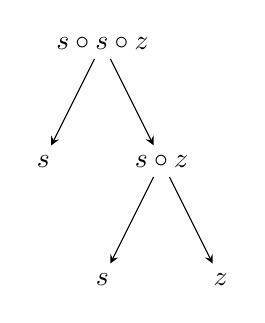
\begin{tikzpicture}[-stealth]
\node { $s \circ \p{s \circ z}$ }
  child { node { $s$ } }
  child { node { $s \circ z$ }
    child { node { $s$ } }
    child { node { $z$ } }
  }
;
\end{tikzpicture}
\caption[]{$\p{s \circ \p{s \circ z}}\p{x} = 3$ for all $x \in S$.}
\end{subfigure}
%
\begin{subfigure}{0.49\textwidth}
\centering
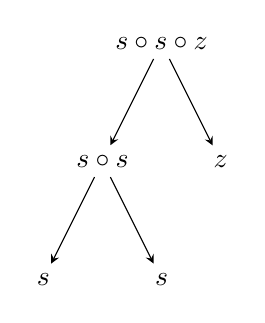
\begin{tikzpicture}[-stealth]
\node { $\p{s \circ s} \circ z$ }
  child { node { $s \circ s$ }
    child { node { $s$ } }
    child { node { $s$ } }
  }
  child { node { $z$ } }
;
\end{tikzpicture}
\caption[]{$\p{\p{s \circ s} \circ z}\p{x} = 3$ for all $x \in S$.}
\end{subfigure}
\caption[]{An illustration of $\mathcal{T}_\mathcal{PD}\p{s \circ \p{s \circ
z}}$ and $\mathcal{T}_\mathcal{PD}\p{\p{s \circ s} \circ z}$.}
\label{fig:mirror-s-s-z}
\end{figure}

Construction trees are useful for proving properties of function algebras by
\emph{structural induction}. First however, consider a mere proof by \emph{case
analysis}, of a theorem which will simplify further proofs concerning
$\mathcal{PD}$:

\begin{theorem} \label{thm:construction-tree-p} A construction tree
$\mathcal{T}_\mathcal{PD}\p{f}$ is either\begin{enumerate}[label=(\arabic*)]

\item a zero- or successor leaf; or

\item a composition node, with outbound subtrees
$\mathcal{T}_\mathcal{PD}\p{g}$ and $\mathcal{T}_\mathcal{PD}\p{h_1} \ldots,
\mathcal{T}_\mathcal{PD}\p{h_m}$, where $f = g \circ \seq{h_1, \ldots, h_m}$.

\end{enumerate}\end{theorem}

\begin{proof} By case analysis of the structure of
$\mathcal{T}_\mathcal{PD}\p{f}$.  There are two
cases:\begin{enumerate}[label=(\arabic*)]

\item $\mathcal{T}_\mathcal{PD}\p{f}$ is an $i$ leaf, for some initial function
$i \in \mathcal{PD}_I$, where $f = i$.

By definition of $\mathcal{PD}_I$, $i$ must either be a zero or successor
function.

Case (1) of the theorem follows.

\item $\mathcal{T}_\mathcal{PD}\p{f}$ is an $op$ node, for some operation $op
\in \mathcal{PD}_O$, having the outbound subtrees
$\mathcal{T}_\mathcal{PD}\p{g_1}, \ldots, \mathcal{T}_\mathcal{PD}\p{g_n}$,
where $f = o\p{g_1, \ldots, g_n}$.

By definition of $\mathcal{PD}_O$, $op$ must be a composition operation. We
must have $f = g_1 \circ \seq{g_2,\ldots, g_n}$. Let $g = g_1$, and let $h_1 =
g_2$, \ldots, $h_m = g_n$.

Case (2) of the theorem follows.\end{enumerate}\end{proof}

Noting that $\mathcal{PD}$ is ``number-valued'' admits a proof by
\emph{structural induction}:

\begin{definition} A function $f$ is \textbf{$T$-valued} iff the codomain of
$f$ is $T$; $f$ is \textbf{number-valued} iff $f$ is $\mathbb{N}$-valued.
Similarly, a function class $\mathcal{C}$ is $T$-valued iff every $f \in
\mathcal{C}$ is $T$-valued; $\mathcal{C}$ is number-valued iff $\mathcal{C}$ is
$\mathbb{N}$-valued. A $T$-valued function algebra \textbf{generates} elements
of $T$ --- a number-valued function algebra generates natural numbers.
\index{$T$-valued!function} \index{$T$-valued!function algebra}
\index{number-valued!function} \index{number-valued!function
algebra}\end{definition}

\begin{theorem} \label{thm:p-number-valued} $\mathcal{PD}$ is number-valued.
\end{theorem}

\begin{proof} By induction on the structure of $\mathcal{T}_\mathcal{PD}\p{f}$.
There are two cases:\begin{enumerate}[label=(\arabic*)]

\item $\mathcal{T}_\mathcal{PD}\p{f}$ is a zero- or successor leaf.

Both the zero and successor functions are number-valued.

\item $\mathcal{T}_\mathcal{PD}\p{f}$ is a composition node, having the
outbound subtrees $\mathcal{T}_\mathcal{PD}\p{g}$ and
$\mathcal{T}_\mathcal{PD}\p{h_1}, \ldots \mathcal{T}_\mathcal{PD}\p{h_m}$,
where $f = g \circ \seq{h_1, \ldots, h_m}$.

By IH, $g$ is number-valued. By definition of composition, the codomain of $f =
g \circ \seq{h_1, \ldots h_m}$ is the codomain of $g$, so $f$ must be
number-valued.\end{enumerate}\end{proof}

In attempt to explore the limits of $\mathcal{PD}$, note that every function in
$\mathcal{PD}$ is merely an intricate composition of zero and successor
functions:

\begin{theorem} \label{thm:p-tree-leafs} A construction tree
$\mathcal{T}_\mathcal{PD}\p{f}$ has $i+j$ leafs, for some $i,j \in \mathbb{N}$,
$i$ of which are zero leafs, and $j$ of which are successor leafs.
\end{theorem}

\begin{proof} By \refDef{function-algebra-p} and \refDef{construction-tree},
every leaf of $\mathcal{T}_\mathcal{PD}\p{f}$ is either a zero- or successor
leaf. $\mathcal{T}_\mathcal{PD}\p{f}$ is a finite tree. It is well-known that a
finite tree has a finite number of leafs. WLOG, let
$\mathcal{T}_\mathcal{PD}\p{f}$ have $i+j$ leafs, for some $i, j \in
\mathbb{N}$, $i$ of which are zero leafs, and $j$ of which are successor
leafs.\end{proof}

Consider first the case with no zero leafs. That is, consider those $f \in
\mathcal{PD}$ which are merely an intricate composition of successor functions.
It holds for such an $f$, that for all $n \in \mathbb{N}$, we have
$f\p{n}=n+j$, where $j$ is the number of (successor) leafs in
$\mathcal{T}_\mathcal{PD}\p{f}$.

For instance, both $\p{s \circ \p{s \circ s}}$ and $\p{\p{s \circ s} \circ s}$
yield the third successor of the input. The respective construction trees are
mirrored in \refFigure{mirror-s-s-s}.

\begin{figure}[h!]
\centering
%
\begin{subfigure}{0.49\textwidth}
\centering
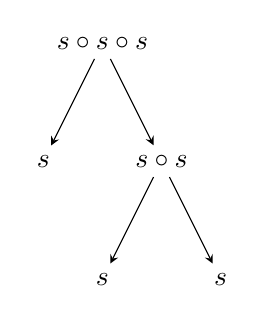
\begin{tikzpicture}[-stealth]
\node { $s \circ \p{s \circ s}$ }
  child { node { $s$ } }
  child { node { $s \circ s$ }
    child { node { $s$ } }
    child { node { $s$ } }
  }
;
\end{tikzpicture}
\caption[]{$\p{s \circ \p{s \circ s}}\p{x} = x + 3$ for all $x \in
\mathbb{N}$.}
\end{subfigure}
%
\begin{subfigure}{0.49\textwidth}
\centering
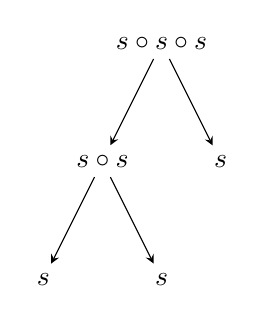
\begin{tikzpicture}[-stealth]
\node { $\p{s \circ s} \circ s$ }
  child { node { $s \circ s$ }
    child { node { $s$ } }
    child { node { $s$ } }
  }
  child { node { $s$ } }
;
\end{tikzpicture}
\caption[]{$\p{\p{s \circ s} \circ s}\p{x} = x + 3$ for all $x \in
\mathbb{N}$.}
\end{subfigure}
\caption[]{An illustration of $\mathcal{T}_\mathcal{PD}\p{s \circ \p{s \circ
s}}$ and $\mathcal{T}_\mathcal{PD}\p{\p{s \circ s} \circ s}$.}
\label{fig:mirror-s-s-s}
\end{figure}

\begin{lemma} \label{lem:p-no-zero} If $\mathcal{T}_\mathcal{PD}\p{f}$ has
$i=0$ zero leafs, and $j$ successor leafs, then $f : \mathbb{N} \rightarrow
\mathbb{N}$ and $f\p{x} = x + j$, for all $x \in \mathbb{N}$. \end{lemma}

\begin{proof} By induction on the structure of $\mathcal{T}_\mathcal{PD}\p{f}$.
There are two cases:\begin{enumerate}[label=(\arabic*)]

\item $\mathcal{T}_\mathcal{PD}\p{f}$ is a zero- or successor leaf.

We assumed $i = 0$, so $\mathcal{T}_\mathcal{PD}\p{f}$ must be a successor
leaf, i.e. $j=1$.

By definition of the successor function, $f\p{x} = x + 1$, for all $x \in
\mathbb{N}$.

\item $\mathcal{T}_\mathcal{PD}\p{f}$ is a composition node, having the
outbound subtrees $\mathcal{T}_\mathcal{PD}\p{g}$ and
$\mathcal{T}_\mathcal{PD}\p{h_1}, \ldots \mathcal{T}_\mathcal{PD}\p{h_m}$,
where $f = g \circ \seq{h_1, \ldots, h_m}$.

By the preceding lemma, $\mathcal{T}_\mathcal{PD}\p{f}$ has $\p{i+j}$ leafs,
for some $i, j \in \mathbb{N}$, $i$ of which are zero leafs, and $j$ of which
are successor leafs.  Similarly, let $\mathcal{T}_\mathcal{PD}\p{g}$ have
$\p{i_g + j_g}$ leafs, and likewise for $h_1,\ldots,h_m$.

It is well-known that the number of (zero or successor) leafs in a tree rooted
at an internal node, is equal to the sum of the number of (zero or successor)
leafs in the outbound subtrees. We must have $i = i_g + i_{h_1} + \cdots +
i_{h_m}$ and $j = j_g + j_{h_1} + \cdots + j_{h_m}$.

We assumed $i = 0$, and so $i = i_g = i_{h_1} = \cdots = i_{h_m} = 0$. The
number of (successor) leafs in $\mathcal{T}_\mathcal{PD}\p{f}$ is therefore
simply $j = j_g + j_{h_1} + \cdots + j_{h_m}$.

By IH, $g : \mathbb{N} \rightarrow \mathbb{N}$ and $g\p{x} = x + j_g$, for all
$x \in \mathbb{N}$, where $\mathcal{T}_\mathcal{PD}\p{g}$ has $i_g = 0$ zero
leafs, and $j_g$ successor leafs. Similarly for $h_1, \ldots, h_m$.

By definition of composition, we must have $m=1$, $f : \mathbb{N} \rightarrow
\mathbb{N}$, and\begin{align*}
%
f\p{x}  &= g\p{h_1\p{x}} \\
        &= g\p{x + j_{h_1}} \\
        &= \p{x + j_{h_1}} + j_g \\
        &= x + j_g + j_{h_1} \\
        &= x + \p{j_g + j_{h_1} + \cdots + j_{h_m}} \\
        &= x + j \text{, for all $x \in \mathbb{N}$.}
%
\end{align*}\end{enumerate}\end{proof}

Consider now the case with at least one zero leaf. Such a function $f \in
\mathcal{PD}$ is a constant function, which always yields a particular natural
number, which is less than or equal to the number of successor leafs in
$\mathcal{T}_\mathcal{PD}\p{f}$.

A case with the exactly one zero leaf as the right-most leaf of the
construction tree, has already been illustrated in \refFigure{mirror-s-s-z}. A
case with multiple zero leafs, and a case with the only zero leaf being not the
right-most leaf, are illustrated in \refFigure{fancy-zero-leafs}.

\begin{figure}[h!]
\centering
%
\begin{subfigure}{0.49\textwidth}
\centering
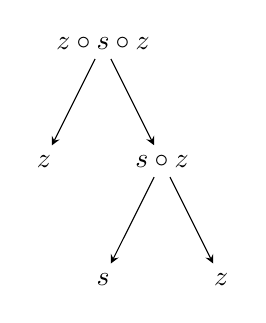
\begin{tikzpicture}[-stealth]
\node { $z \circ \p{s \circ z}$ }
  child { node { $z$ } }
  child { node { $s \circ z$ }
    child { node { $s$ } }
    child { node { $z$ } }
  }
;
\end{tikzpicture}
\caption[]{$\p{z \circ \p{s \circ z}}\p{x} = 0$ for all $x \in S$.}
\end{subfigure}
%
\begin{subfigure}{0.49\textwidth}
\centering
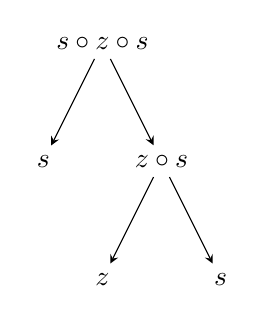
\begin{tikzpicture}[-stealth]
\node { $s \circ \p{z \circ s}$ }
  child { node { $s$ } }
  child { node { $z \circ s$ }
    child { node { $z$ } }
    child { node { $s$ } }
  }
;
\end{tikzpicture}
\caption[]{$\p{s \circ \p{z \circ s}}\p{x} = 1$ for all $x \in S$.}
\end{subfigure}
%
\caption[]{An illustration of $\mathcal{T}_\mathcal{PD}\p{z \circ \p{s \circ
z}}$ and $\mathcal{T}_\mathcal{PD}\p{s \circ \p{z \circ s}}$.}
\label{fig:fancy-zero-leafs}
\end{figure}

In general, the following lemma can be stated:

\begin{lemma} \label{lem:p-at-least-one-zero} If
$\mathcal{T}_\mathcal{PD}\p{f}$ has $i > 0$ zero leafs, and $j$ successor
leafs, then $f : S \rightarrow \mathbb{N}$ is a constant function, for some set
$S$, and $f\p{x} \leq j$, for all $x \in S$.  \end{lemma}

\begin{proof} By induction on the structure of $\mathcal{T}_\mathcal{PD}\p{f}$.
There are two cases:\begin{enumerate}[label=(\arabic*)]

\item $\mathcal{T}_\mathcal{PD}\p{f}$ is a zero- or successor leaf.

We assumed $i > 0$, so $\mathcal{T}_\mathcal{PD}\p{f}$ must be a zero leaf,
i.e. $j = 0$.

By definition of the zero function, $f\p{x} = 0$ for all $x \in S$, for some
set $S$.

\item $\mathcal{T}_\mathcal{PD}\p{f}$ is a composition node, having the
outbound subtrees $\mathcal{T}_\mathcal{PD}\p{g}$ and
$\mathcal{T}_\mathcal{PD}\p{h_1}, \ldots, \mathcal{T}_\mathcal{PD}\p{h_m}$,
where $f = g \circ \seq{h_1, \ldots, h_m}$.

By definition of composition, we must have $dom\p{f} = dom\p{h_1} = \cdots =
dom\p{h_m}$. WLOG, let $S=dom\p{h_1}$. Furthermore, by
\refThm{p-number-valued}, $cod\p{f} = \mathbb{N}$, and so we must have $f : S
\rightarrow \mathbb{N}$.

RTS $f\p{x} = g\p{h_1\p{x}, \ldots, h_m\p{x}} \leq j$, for all $x \in S =
dom\p{h_1}$.

It is well-known that the number of (zero or successor) leafs in a tree rooted
at an internal node, is equal to the sum of the number of (zero or successor)
leafs in the outbound subtrees. We must have $i = i_g + i_{h_1} + \cdots +
i_{h_m}$ and $j = j_g + j_{h_1} + \cdots + j_{h_m}$.

We assumed $i > 0$, and so there are two cases for $i_g$:

\begin{enumerate}[label=(\alph*)]

\item If $i_g=0$, then by \refLem{p-no-zero}, $g : \mathbb{N} \rightarrow
\mathbb{N}$ and $g\p{x} = x + j_g$, for all $x \in \mathbb{N}$.

By definition of composition, we must have $dom\p{g} = cod\p{h_1} \times \cdots
\times cod\p{h_m}$. We have $dom\p{g}=\mathbb{N}$. We must have $m=1$, and $i =
i_g + i_{h_1} = i_{h_1} > 0$ and $j = j_g + j_{h_1}$.

By IH on $h_1$ (having $i_{h_1} > 0$), we have $h_1 : S_{h_1} \rightarrow
\mathbb{N}$ is a constant function, for some set $S_{h_1}$, and $h_1\p{x} \leq
j_{h_1}$, for all $x \in S_{h_1}$.

By definition of compostion, we have $f\p{x}  = g\p{h_1\p{x}, \ldots, h_m\p{x}}
= g\p{h_1\p{x}} \leq g\p{j_{h_1}} = j_g + j_{h_1} = j$, for all $x \in S$. The
lemma follows.

\item If $i_g > 0$, then by IH on $g$, we have $g : S_g \rightarrow \mathbb{N}$
is a constant function, for some set $S_g$, and $g\p{x} \leq j_g$, for all $x
\in S_g$.

By definition of composition, we have $f\p{x} = g\p{h_1\p{x},
\ldots, h_m\p{x}} \leq j_g \leq j_g + j_{h_1} + \cdots + j_{h_m} = j$, for all
$x \in S$. The lemma follows.

\end{enumerate}\end{enumerate}\end{proof}

We are ready to state the following theorem regarding the limits of
$\mathcal{PD}$:

\begin{theorem} For any $f \in \mathcal{PD}$, where
$\mathcal{T}_\mathcal{PD}\p{f}$ has $j$ successor leafs,
either\begin{enumerate}[label=(\arabic*)]

\item $f : \mathbb{N} \rightarrow \mathbb{N}$, and $f\p{x} = x+j$ for all $n
\in \mathbb{N}$; or

\item $f : S \rightarrow \mathbb{N}$, for some set $S$, and $f\p{x} = k$, for
all $x \in S$, where $k \leq j$.

\end{enumerate}\end{theorem}

\begin{proof} Follows directly from \refLem{p-no-zero}, and
\refLem{p-at-least-one-zero}. \end{proof}

This is a fairly stringent set of restrictions. As we shall later prove,
$\mathcal{PD}$ is never-the-less, powerful enough to generate all the natural
numbers. $\mathcal{PD}$ is perhaps interesting because it forms a conservative
subset of the first class of a couple interesting hierarchies of
number-theoretic functions. As an example, consider the \emph{primitive
recursive} functions, as contained in the \emph{general recursive} functions,
as well as the slightly more extravagant, \emph{Grzegorczyk hierarchy}.

First however, it is perhaps long overdue to clarify what is meant by
``simple'' initial functions and operations.

Another use of function algebras (and hierarchies) is in the design of
programming languages.  An initial function or operation is considered
``simple'' if it is computable by some ``simple'' machine. A function algebra
is considered ``simple'' if the functions it produces are all computable by
some ``simple'' machine.  A ``simple'' function algebra hereby (informally)
definined a programming language of (only) computable functions.

For instance, the reader will hopefully agree, uniquivocally, that the zero,
successor, composition, and composite functions are all computable, for any
well-known general-purpose (unbounded) model of computation.

% Although $\mathcal{P}$ generates ``only'' natural numbers, it is strong enough
% to generate \emph{all} the natural numbers.

% \begin{theorem} \label{thm:p-generates-all-N} For every $n \in \mathbb{N}$,
% there exists an $f \in \mathcal{P}$, s.t. $f : S \rightarrow \mathbb{N}$ and
% $f\p{x} = n$, for all $x \in S$. \end{theorem}

% \begin{proof} Proof by induction on $n$. There are two cases:

% \begin{enumerate}[label=(\arabic*)]

% \item if $n = 0$, then let $f = z$; and otherwise,

% \item if $n = m + 1$, then by IH, there exists a $g \in \mathcal{P}$, s.t.
% $g\p{x} = m$, for all $x \in S_g$. Let $S=S_g$, and let $f = s \circ g$.
% \end{enumerate} \end{proof}

\section{Some other ``simple'' initial functions}

Before leaving the hearty lands of ``simple'' functions, and diving into the
unwieldy sea of recursion, another ``simple'' initial function is projection:

\subsection{Projection}

\begin{definition} A \textbf{projection} (also called identity)
\textbf{function} $\mathtt{proj}^n_j : S_1 \times \cdots \times S_n \rightarrow
S_j$, is given by $\mathtt{proj}^n_j\p{x_1,\ldots,x_n} = x_j$. \end{definition}

For instance, $\mathtt{proj}^1_1 : S \rightarrow S$ and $\mathtt{proj}^1_1\p{x}
= x$ for all $x \in S$.

\todo{substitution} and \todo{explicit transformation}

\section{Recursion}

The general idea of recursion is perhaps as follows:

\begin{quote}

The value of a \emph{recursively defined} function --- at a \emph{particular}
argument --- depends on the value of \emph{that} function --- at \emph{other}
arguments.

\end{quote}

This notion demands that the value at a particular argument depends on the
value of the function at \emph{other} arguments. This is to avoid an obvious
vicious circle, where the value of a function at a particular argument depends
on the value of that function at that same argument\ldots

Furthermore, this notion demands merely that a function have such a dependency
at a \emph{particular} argument. Demanding such a dependency at all arguments
would again imply a vicious circle. Demanding it at none, would give the
non-recursive functions. Demanding it at some, is adequate.

This latter notice demands that a function definition can partition the domain
into those arguments at which the value of the function is recursively defined,
and those at which the value of the function is determined non-recursively.
Note, such a partitioning alone does not avoid vicious circles in general.

\begin{definition} A function $f$ is \textbf{number-theoretic} iff the domain
of $f$ is $\mathbb{N}$. \end{definition}

For various reasons, the number-theoretic function definitions were perhaps the
first to obtain such a means of partitioning. Indeed, the natural numbers admit
perhaps a very natural interpretation:

\begin{quote}

A natural number is either \emph{zero}, written $0$, or the \emph{successor} of
a natural number $x$, written $x+1$.\cite{dedekind-1888, rose-1984,
odifreddi-1989}.

\end{quote}

% In our case, \refThm{p-generates-all-N} states that $\mathcal{P}$ can
% generate all the natural numbers.

Owing to this intuition, consider first number-theoretic primitive recursion.
The partitioning here is to define the function non-recursively at $0$, and
(perhaps) recursively at any given $x+1$. The value of the function at $x+1$
then (perhaps) depends on the value of \emph{that} function at the ``smaller''
argument, $x$.

This notion of ``natural number'' superimposes an order on the natural numbers,
where $0$ forms a least element. It is this superimposition that guarantees the
absence of a vicious circle with number-theoretic primitive recursion --- the
recursion always ``bottoms out'' at (at most) $0$. This notion will be made
precise later on.

\begin{definition} \label{def:number-theoretic-primitive-recursion} A function
$f : \mathbb{N} \times \mathbf{S} \rightarrow T$ is defined by
\textbf{number-theoretic primitive recursion} from functions $g : \mathbf{S}
\rightarrow T$ and $h : \mathbb{N} \times \mathbf{S} \times T \rightarrow T$,
if $f$ satisfies the following set of equations:\begin{align*}
%
f\p{0, \mathbf{y}} &= g\p{\mathbf{y}}\\
%
f\p{x+1, \mathbf{y}} &= h\p{x,\mathbf{y},f\p{x,\mathbf{y}}}
%
\end{align*}\end{definition}

\begin{remark} The above definition slightly abuses the term
``number-theoretic''. The domain of the function so defined is $\mathbb{N}
\times \mathbf{S}$, not $\mathbb{N}$. It is possible to simulate any
multivariate primitive recursion by a univariate primitive
recursion\cite{rose-1984}.  In modern terms, it is well-known that those
arguments, besides the natural number, can be partially applied --- they play
no role in the recursion.  \end{remark}

\begin{remark} The definition of number-theoretic primitive recursion is very
similar to the classical definition as it appears in \cite{dedekind-1888,
goedel-1944, rose-1984, odifreddi-1989}, among many others. The main difference
is that classically, we let $\mathbf{S}=\mathbb{N}^k$ for some $k \in
\mathbb{N}$, and let $T = \mathbb{N}$. That is, we consider only perhaps
``purely'' number-theoretic and number-valued functions. \end{remark}

\begin{definition} A \textbf{number-theoretic primitive recursion operation}
%
$$\mathtt{nprec} : \p{\mathbf{S} \rightarrow T} \rightarrow \p{\mathbb{N}
\times \mathbf{S} \times T \rightarrow T} \rightarrow \p{\mathbb{N} \times
\mathbf{S} \rightarrow T},$$
%
takes as input the functions $g : \mathbf{S} \rightarrow T$ and $h : \mathbb{N}
\times \mathbf{S} \times T \rightarrow T$, and yields as output a function $f :
\mathbb{N} \times \mathbf{S} \rightarrow T$, defined by number-theoretic
primitive recursion from $g$ and $h$.\end{definition}

\begin{definition} Let $\mathcal{PR}$ be a \textbf{primitive recursive function
algebra}, extending $\mathcal{P}$ with the projection initial function and
number-theoretic primitive recursion operation.\end{definition}

\section{Some functions in $\mathcal{PR}$}

It has earlier been noted that another good use of function algebras is in the
design of programming languages. The class of primitive recursive functions is
claimed to be expressive enough to express a wide range of mathematical
functions. This section exemplifies how various well-known mathematical
functions can be given in terms of functions in $\mathcal{PR}$.

\subsection{Predecessor}

Having a successor function, it is natural to consider a (total) predecessor
function, $\mathtt{pred} : \mathbb{N} \times () \rightarrow \mathbb{N}$.
Mathematically, predecessor can be given as follows:\begin{align*}
%
\mathtt{pred}\p{0,()} &= 0 \\
%
\mathtt{pred}\p{x+1,()} &= x
%
\end{align*}

Predecessor function as given above, partitions the domain as in
number-theoretic primitive recursion (with $S = ()$), and so predecessor can be
expressed as $\mathtt{nprec}\p{g,h}$, for some suitable $g$ and $h$:

\begin{enumerate}[label=(\arabic*)]

\item We must have $g\p{} = 0$. That is, $g$ must yield the constant value $0$.

Let  $g=\mathtt{z}$.

\item We must have $h\p{x,(),\mathtt{pred}\p{n,()}}=x$. That is, $h$ must yield
the first projection of the input triple.

Let $h = \mathtt{proj^3_1}$.

\end{enumerate}

The equation follows:\begin{align*}
%
\mathtt{pred} = \mathtt{nprec}\p{\mathtt{z}, \mathtt{proj}^3_1}
%
\end{align*}

\subsection{Addition}

It is perhaps natural to consider addition, $\mathtt{sum} : \mathbb{N} \times
\mathbb{N} \rightarrow \mathbb{N}$, as defined in terms of an iterated
application of a successor function, an adequate number of times.
Mathematically, addition can be given as follows:\begin{align*}
%
\mathtt{sum}\p{0, y} &= y \\
%
\mathtt{sum}\p{x+1, y} &= \mathtt{sum}\p{x,y} + 1 
%
\end{align*}

Addition as given above, partitions the domain as in number-theoretic primitive
recursion (with $S = \mathbb{N}$), and so addition can be expressed as
$\mathtt{nprec}\p{g,h}$, for some suitable $g$ and $h$:

\begin{enumerate}[label=(\arabic*)]

\item We must have $g\p{y} = y$. That is, $g$ must yield the input value.

Let $g = \mathtt{proj}^1_1$.

\item We must have $h\p{x,y,\mathtt{sum}\p{x,y}} = \mathtt{sum}\p{x,y} + 1$.
That is, $h$ must yield the successor of the 3\textsuperscript{rd} projection
of the input triple.

Let $h = \mathtt{s} \circ \mathtt{proj}^3_3$.

\end{enumerate}

The equation follows:\begin{align*}
%
\mathtt{sum} = \mathtt{nprec}\p{\mathtt{proj}^1_1, \mathtt{s} \circ
\mathtt{proj}^3_3}
%
\end{align*}

\subsection{Multiplication}

In lieu of addition as iterated successor, it is perhaps natural to consider
multiplication, $\mathtt{mult} : \mathbb{N} \times \mathbb{N} \rightarrow
\mathbb{N}$, as iterated addition. Mathematically, multiplication can be given
as follows:\begin{align*}
%
\mathtt{mult}\p{0, y} &= 0 \\
%
\mathtt{mult}\p{x+1,y} &= \mathtt{sum}\p{y, \mathtt{mult}\p{x,y}}
%
\end{align*}

Multiplication as given above, partitions the domain as in number-theoretic
primitive recursion (with $S = \mathbb{N}$), and so multiplication can be
expressed as $\mathtt{nprec}\p{g,h}$, for some suitable $g$ and $h$:

\begin{enumerate}[label=(\arabic*)]

\item We must have $g\p{y} = 0$. That is, $g$ must yield the constant value $0$.

Let $g = \mathtt{z}$.

\item We must have $h\p{x,y,\mathtt{mult}\p{x,y}} =
\mathtt{sum}\p{y,\mathtt{mult}\p{x,y}}$. That is, $h$ must yield $\mathtt{sum}$
applied to the 2\textsuperscript{nd} and 3\textsuperscript{rd} projections of
the input triple.

Let $h = \mathtt{sum} \circ \seq{\mathtt{proj}^3_2, \mathtt{proj}^3_3}$.

\end{enumerate}

The equation follows:\begin{align*}
%
\mathtt{mult} = \mathtt{nprec}\p{\mathtt{z}, \mathtt{sum} \circ
\seq{\mathtt{proj}^3_2, \mathtt{proj}^3_3}}
%
\end{align*}

\subsection{Exponentiation}

In lieu of multiplication as iterated addition, it is perhaps natural to
consider exponentiation, $\mathtt{exp} : \mathbb{N} \times \mathbb{N}
\rightarrow \mathbb{N}$, as iterated multiplication.  Mathematically,
exponentiation can be given as follows:\begin{align*}
%
\mathtt{exp}\p{0, y} &= 1 \\
%
\mathtt{exp}\p{x+1, y} &= \mathtt{mult}\p{y, \mathtt{exp}\p{x,y}}
%
\end{align*}

Exponentiation as given above, partitions the domain as in number-theoretic
primitive recursion (with $S = \mathbb{N}$), and so exponentiation can be
expressed as $\mathtt{nprec}\p{g,h}$, for some suitable $g$ and $h$:

\begin{enumerate}[label=(\arabic*)]

\item We must have $g\p{y} = 1$. That is, $g$ must yield the constant value $1$.

Let $g = \mathtt{s} \circ \mathtt{z}$.

\item We must have $h\p{x,y,\mathtt{exp}\p{x,y}} = \mathtt{mult}\p{y,
\mathtt{exp}\p{x,y}}$. That is, $h$ must yield $\mathtt{mult}$ applied to the
2\textsuperscript{nd} and 3\textsuperscript{rd} projections of the input
triple.

Let $h = \mathtt{mult} \circ \seq{\mathtt{proj}^3_2,\mathtt{proj}^3_3}$.

\end{enumerate}

The equation follows:\begin{align*}
%
\mathtt{exp} = \mathtt{nprec}\p{\mathtt{s} \circ \mathtt{z}, \mathtt{mult}
\circ \seq{\mathtt{proj}^3_2, \mathtt{proj}^3_3}}
%
\end{align*}

\subsection{Factorial}

A go-to function in any new and exciting programming language is perhaps the
factorial function, $\mathtt{fact} : \mathbb{N} \times () \rightarrow
\mathbb{N}$.  Mathematically, it can be given as follows:\begin{align*}
%
\mathtt{fact}\p{0,()} &= 1 \\
%
\mathtt{fact}\p{x+1,()} &= \mathtt{mult}\p{\p{x+1}, \mathtt{fact}\p{x,()}}
%
\end{align*}

Again, the factorial function partitions the domain as in number-theoretic
primitive recursion (with $S = ()$), and so the factorial function can be expressed as
$\mathtt{nprec}\p{g,h}$ for some suitable $g$ and $h$:

\begin{enumerate}[label=(\arabic*)]

\item We must have $g\p{} = 1$. That is, $g$ must yield a constant value $1$.

Let $g = \mathtt{s} \circ \mathtt{z}$.

\item We must have $h\p{x,(),\mathtt{fact}\p{x,()}} = \mathtt{mult}\p{\p{x+1},
\mathtt{fact}\p{x,()}}$. That is, $h$ must yield $\mathtt{mult}$ applied to the
successor of the 1\textsuperscript{st} projection, and the
3\textsuperscript{rd} projection of the input triple.

Let $h = \mathtt{mult} \circ \seq{\mathtt{z} \circ \mathtt{proj}^3_1,
\mathtt{proj^3_3}}$.

\end{enumerate}

The equation follows:\begin{align*}
%
\mathtt{fact} = \mathtt{nprec}\p{\mathtt{s} \circ \mathtt{z},
\mathtt{mult} \circ \seq{\mathtt{z} \circ \mathtt{proj}^3_1, \mathtt{proj^3_3}}}
%
\end{align*}

\subsection{Tetration and beyond}

Tetration, $\mathtt{exp}^2 : \mathbb{N} \times \mathbb{N} \rightarrow
\mathbb{N}$, is iterated exponentiation. Mathematically, tetration can be given
as follows:\begin{align*}
%
\mathtt{exp}^2\p{0,y} &= 1 \\
%
\mathtt{exp}^2\p{x+1, y} &= \mathtt{exp}\p{y,\mathtt{exp}^2\p{x,y}}
%
\end{align*}

Tetration as given above, partitions the domain as in number-theoretic
primitive recursion (with $S = \mathbb{N}$), and so tetration can be expressed
as $\mathtt{nprec}\p{g,h}$, for some suitable $g$ and $h$:

\begin{enumerate}[label=(\arabic*)]

\item We must have $g\p{y} = 1$. That is, $g$ must yield the constant value $1$.

Let $g = \mathtt{s} \circ \mathtt{z}$.

\item We must have $h\p{x,y,\mathtt{exp}^2\p{x,y}} = \mathtt{exp}\p{y,
\mathtt{exp}^2\p{x,y}}$. That is, $h$ must yield $\mathtt{exp}$ applied to the
2\textsuperscript{nd} and 3\textsuperscript{rd} projections of the input
triple.

Let $h = \mathtt{exp} \circ \seq{\mathtt{proj}^3_2,\mathtt{proj}^3_3}$.

\end{enumerate}

The equation follows:\begin{align*}
%
\mathtt{exp}^2 = \mathtt{nprec}\p{\mathtt{s} \circ \mathtt{z}, \mathtt{exp}
\circ \seq{\mathtt{proj}^3_2, \mathtt{proj}^3_3}}
%
\end{align*}

If we let $\mathtt{exp}^0 = \mathtt{mult}$ (and let $\mathtt{exp}^1 =
\mathtt{exp}$), it is straight-forward to generalise from $\mathtt{exp}^1$ and
$\mathtt{exp}^2$ to $\mathtt{exp}^k$ for any given $k \in
\mathbb{N}$:\begin{align*}
%
\mathtt{exp}^0 &= \mathtt{mult} \\
%
\mathtt{exp}^{k+1} &= \mathtt{nprec}\p{\mathtt{s} \circ \mathtt{z},
\mathtt{exp}^k \circ \seq{\mathtt{proj}^3_2, \mathtt{proj}^3_3}}
%
\end{align*}

Although this seems to take the shape of a primitive recursion wrt. $k$, this
is a (number-theoretic) primitive recursion over functions (construction trees)
rather than over values --- a higher-order primitive recursion. This is perhaps
better illustrated if we consider the purely mathematical definition of
$\mathtt{exp}^{k+1}$:\begin{align*}
%
\mathtt{exp}^{k+1}\p{0,y} &= 1 \\
%
\mathtt{exp}^{k+1}\p{x+1,y} &= \mathtt{exp}^k\p{y,\mathtt{exp}^{k+1}\p{x,y}}
%
\end{align*}

Reshaping this (trivially) as a ternary function $\mathtt{arr} : \mathbb{N}
\times \mathbb{N} \times \mathbb{N} \rightarrow \mathbb{N}$, so that
$\mathtt{exp}^{k+1}\p{x,y} = \mathtt{arr}\p{k+1,x,y}$, we get the
following:\begin{align*}
%
\mathtt{arr}\p{k+1, 0,y} &= 1 \\
%
\mathtt{arr}\p{k+1,x+1,y} &= \mathtt{arr}\p{k,y,\mathtt{arr}\p{k+1,x,y}}
%
\end{align*}

Clearly, a base case is missing for if $k$ reaches $0$.  Noting that we had let
$\mathtt{exp}^0 = \mathtt{mult}$, we get the following complete
definition:\begin{align*}
%
\mathtt{arr}\p{0,x,y} &= \mathtt{mult}\p{x,y} \\
%
\mathtt{arr}\p{k+1, 0,y} &= 1 \\
%
\mathtt{arr}\p{k+1,x+1,y} &= \mathtt{arr}\p{k,y,\mathtt{arr}\p{k+1,x,y}}
%
\end{align*}

\begin{remark} The name $\mathtt{arr}$ is a reference to Knuth's up-arrow
notation\cite{knuth-1976}. Knuth had let $x \uparrow y = \mathtt{exp}\p{x,y}$,
$x \uparrow \uparrow y = \mathtt{exp}^2\p{x,y}$, and more generally, $x
\underbrace{\uparrow \cdots \uparrow}_{\text{$k$ times}} y =
\mathtt{exp}^k\p{x,y} = \mathtt{arr}\p{k,x,y}$. \end{remark}

\section{A function not in $\mathcal{PR}$}

\todo{Ackermann function}

% That is, let the first argument of $f$ (the recurrence argument) be a natural
% number, with the remaining arguments (if any) forming an element of some set
% $\mathbf{A}$, and let $f$ yield a value of some set $B$. 

% Perhaps the simplest form of recursion is that of iteratively applying a
% particular function a given number of times.  That is, an $f : S \rightarrow
% S$ is defined by \emph{pure iteration} from a $g : S \rightarrow S$ and $n
% \in \mathbb{N}$, by $f\p{x} = g^n\p{x}$. Although pure iteration, coupled
% with a few hearty initial functions is a powerful operation\cite{rose-1984},
% it is about time to jump to something a bit more handy.

% primitive recursive functions before Grzegorczyk.

% primitive recursion is rather powerful from a complexity-theoretic point of
% view: the sequence of prime numbers is primitive recursive.

% predecessor is primitive recursive.

% definition by = scheme

% To get off the ground we need to employ the scheme of definition by
% recursion.  In a recursive scheme, a function is still given by a set of
% equations, but the function being defined also appears on the right-hand side
% of the equality sign.

% Loops are not allowed in a construction tree.

% Unfortunately, such a recursion does not terminate. A \emph{primitive} form
% of recursion 

% Any construction tree is finite.

% \todo{A \textbf{hierarchy of functions}, successively takes a class of
% functions as initial functions and closes it under a set of operations.}

% That is, for all $f
%\in \mathcal{C}_I$, we have $f \in \mathcal{C}$, and for all $g \in \mathcal{C}_O$, 

% initial functions: the set of functions which form the leafs of a computation
% tree; it is however up to interepretation what one regards as the leafs of
% this computation tree, except for perhaps the 0-ary functions, which lead to
% no subsequent function calls. On the other hand, our definition of the
% successor function also leads to no 

% in classical recursion theory, we define functions over the natural numbers;
% we designate some functions as initial, and others as operators. The
% operators combine the initial functions and operators to construct new
% values. This induces a construction tree. Given sufficiently simple initial
% functions, and sufficiently simple constructions -- we can superimpose a
% computation model on top of a function algebra. Here, sufficiently simple
% means computable, and typically, easily computable.
